\vspace{1.5pc}
\section[Domain Penelitian]{Domain Penelitian}
\begin{spacing}{1.5}
	Domain penelitian meliputi wilayah perairan Aceh, Selat Malaka, Bagian Laut Cina Selatan dengan koordinat $-6.22^\circ-6.8^\circ$ LU dan $89.1^\circ-106.6^\circ$ BT (lihat Gambar \ref{fig:domain}) dan Teluk Benggala dengan koordinat $5.5^\circ-24.6^\circ$ LU dan $78.2^\circ-96.7^\circ$ BT (lihat Gambar \ref{fig:domain_1}). Data batimetri untuk domain penelitian diperoleh dari SRTM15+ \href{https://topex.ucsd.edu/pub/archive/srtm15/V1/}{(https://topex.ucsd.edu/)} - kisi elevasi global yang diperbarui pada interval pengambilan sampel spasial 15 arc-second (ukuran piksel $\sim 500 \times 500$ m di ekuator) \shortcite{Tozer2019}. Penelitian ini dilakukan dengan mengkaji variabilitas lapisan vertikal berdasarkan data meteorology dan aplikasinya di beberapa domain penelitian. Pertimbangan domain ini bertujuan untuk melihat keberlakukan secara umum, terhadap teori iklim dan MLD, oleh karena itu perlu diterapkan aplikasi di beberapa tempat seperti: BoB, Perairan Aceh, Selat Malaka, dan Bagian Laut Cina Selatan.
	\begin{figure}[H]
		\centering
		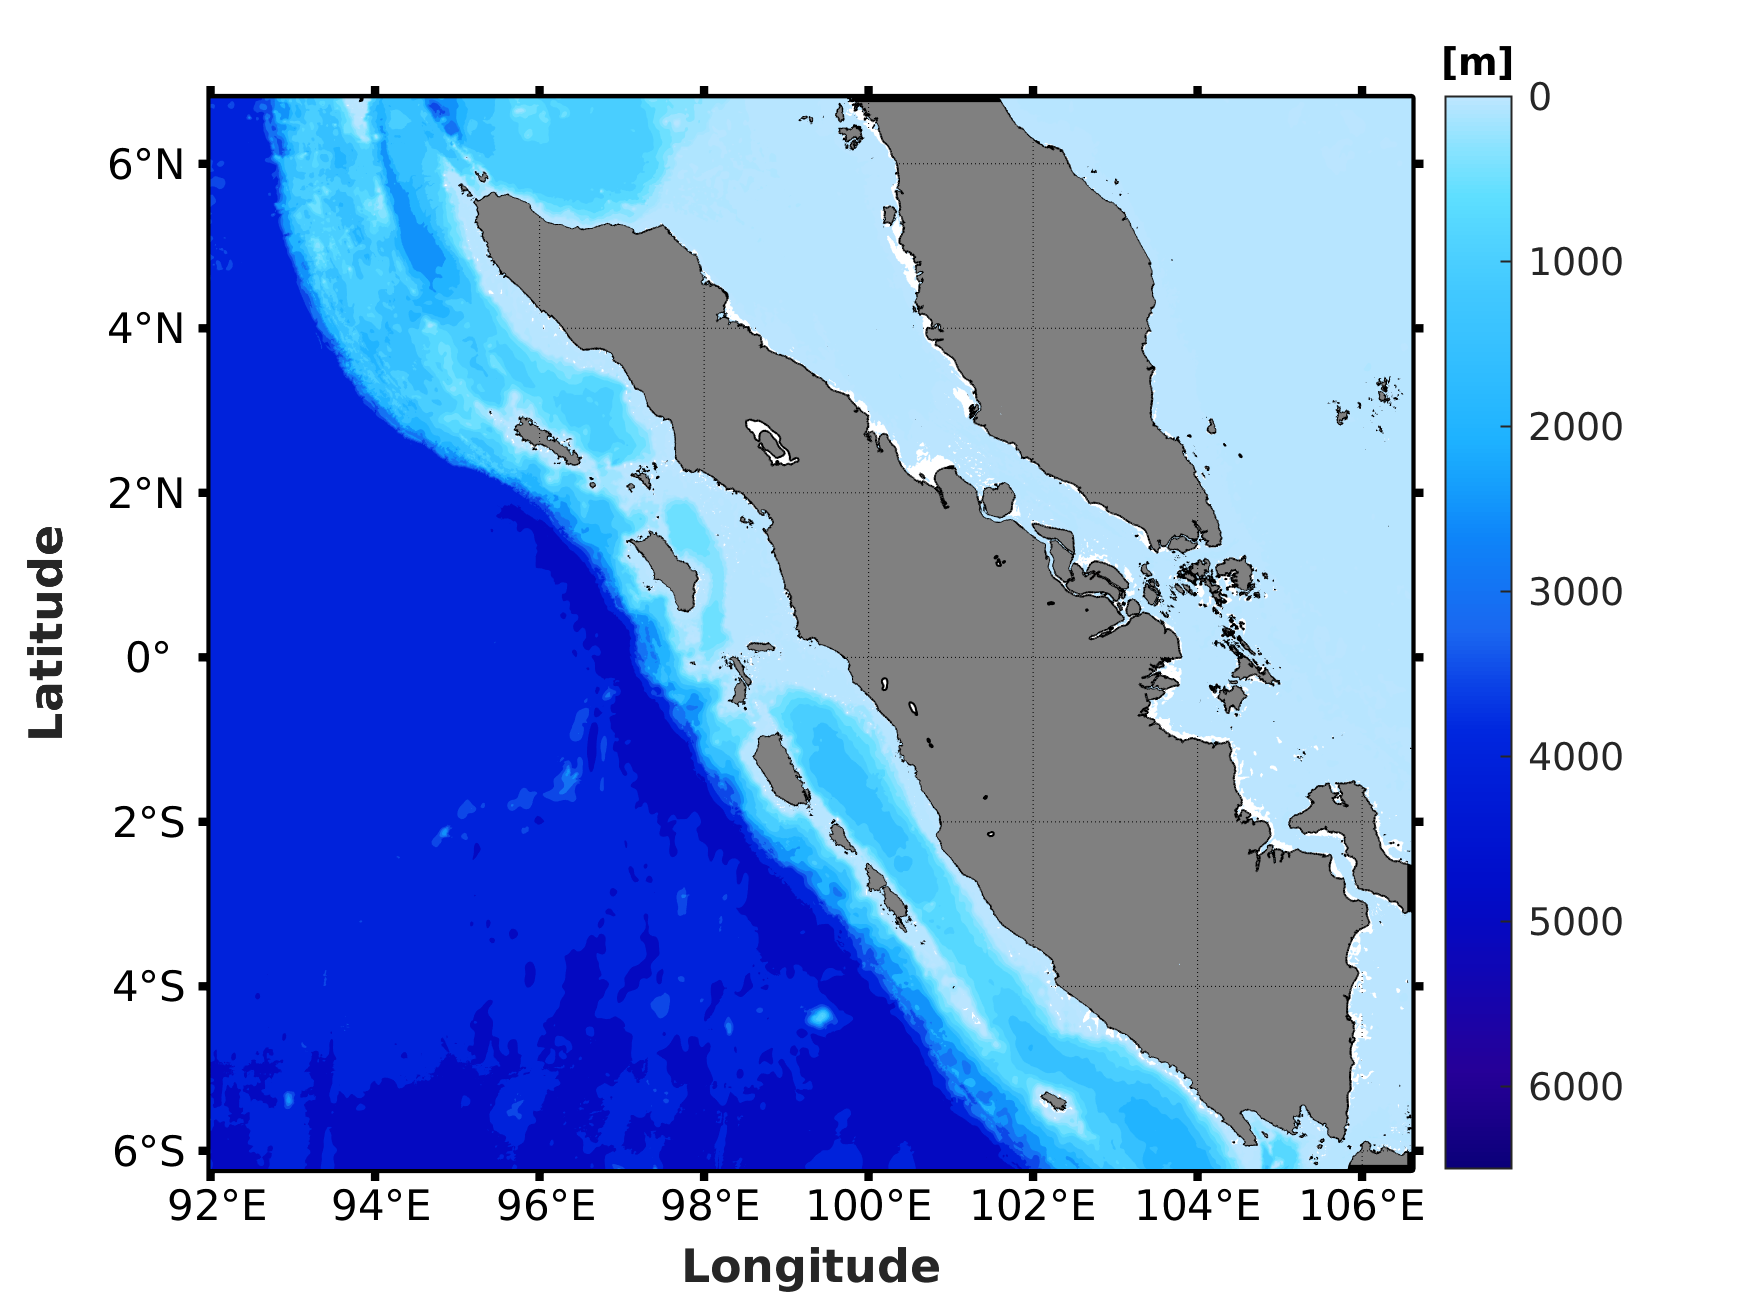
\includegraphics[width=12cm]{contents/Topo_1}
		\caption{Data batimetri domain perairan Aceh, Selat Malaka, Bagian Laut Cina Selatan, dicuplik dari SRTM15+}
		\label{fig:domain}
	\end{figure}
	\begin{figure}[H]
		\centering
		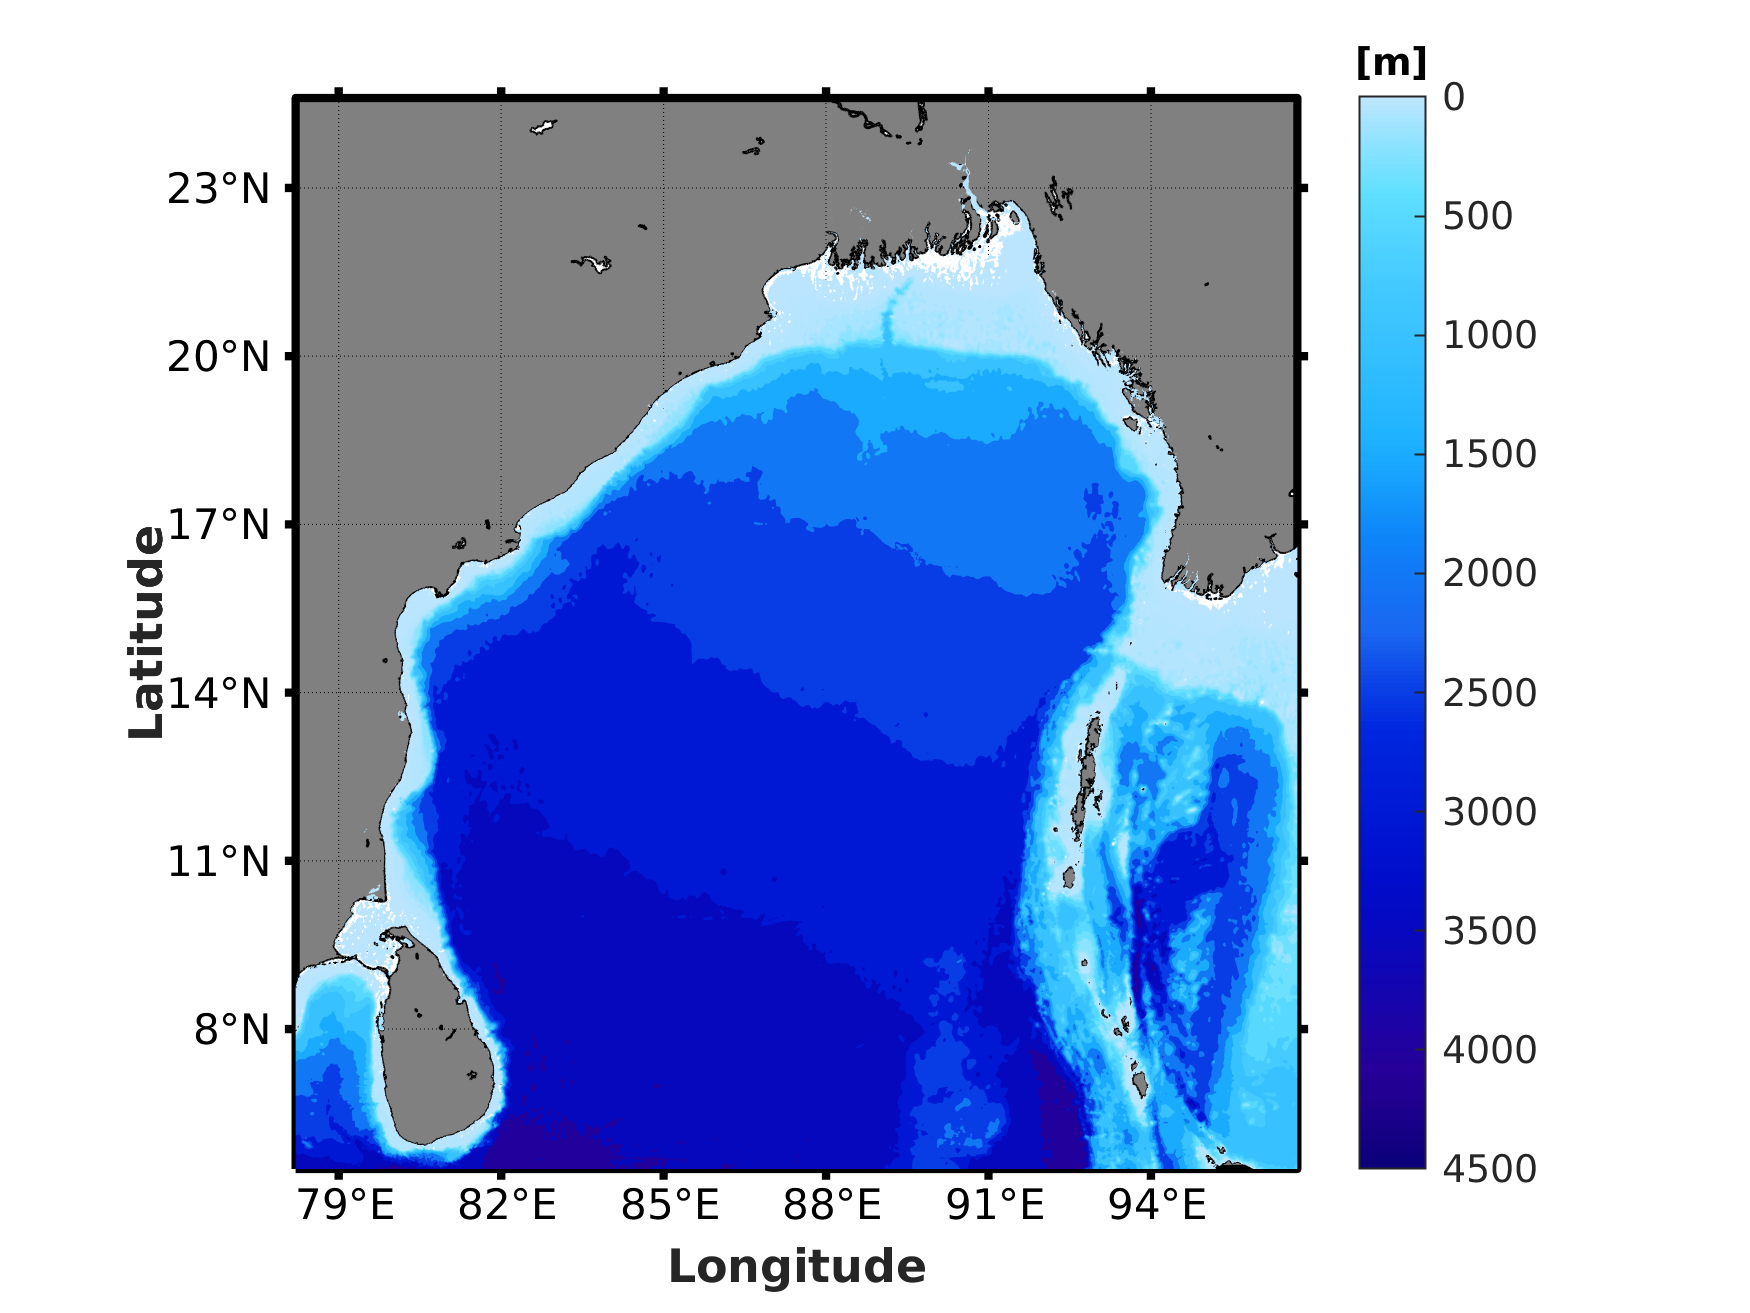
\includegraphics[width=12cm]{contents/Topo_2}
		\caption{Data batimetri domain Teluk Benggala, dicuplik dari SRTM15+}
		\label{fig:domain_1}
	\end{figure}
%	\begin{table}[htp]
%		\centering
%		\caption{Stasiun Penelitian}
%		\label{table:stasiun}
%		\begin{tabular}{ll}
%			Stasiun & Koordinat \\ \hline
%			$1$ & $3.25^\circ \text{LU}, 94^\circ \text{BT}$ \\
%			$2$ & $3.25^\circ \text{LU}, 95^\circ \text{BT}$ \\
%			$3$ & $3.25^\circ \text{LU}, 97^\circ \text{BT}$ \\
%			$4$ & $4.5^\circ \text{LU}, 94^\circ \text{BT}$ \\
%			$5$ & $4.5^\circ \text{LU}, 95^\circ \text{BT}$ \\
%			$6$ & $6^\circ \text{LU}, 94^\circ \text{BT}$ \\
%			$7$ & $6^\circ \text{LU}, 95^\circ \text{BT}$ \\
%			$8$ & $6^\circ \text{LU}, 97^\circ \text{BT}$ 
%		\end{tabular}
%	\end{table}
\end{spacing}
\vspace{-1pc}
\section[Data Penelitian]{Data Penelitian}
\begin{spacing}{1.5}
\vspace{-1pc}
\subsection[Data Oseanografi]{Data Oseanografi}
	Data oseanografi yang digunakan adalah data arus permukaan, serta data temperatur dari NEMO (\textit{Nucleus for European Modeling of the Ocean}) yang merupakan salah satu model sirkulasi laut (OGCM) yang menggunakan model numerik tiga dimensi Navier-Stokes. Model NEMO adalah model komputasi resolusi tinggi yang digunakan untuk kegiatan penelitian dan layanan peramalan dalam oseanografi dan klimatologi, yang dikembangkan secara berkelanjutan sejak 2008 oleh konsorsium Eropa yang terdiri dari 5 institusi (CMCC | CNRS | Mercator Ocean | Met Office | NERC). Hal ini dimaksudkan untuk menjadi alat yang fleksibel untuk mempelajari fenomena fisik dan biogeokimia dalam sirkulasi laut, serta interaksinya dengan komponen sistem iklim Bumi, pada berbagai skala ruang dan waktu \shortcite{madec_gurvan_2022_6334656}. 
	
	Penelitian ini menggunakan data output model NEMO (\href{https://www.nemo-ocean.eu/}{https://www.nemo-ocean.eu/}) untuk data analisis global temperatur tiga dimensi yang didownload dari website \href{https://resources.marine.copernicus.eu/products}{CMEMS} selama 12 bulan (Januari - Desember) tahun 2021.  Dalam analisis kami, resolusi data output yang digunakan adalah dx = dy = 5 menit pada bidang horizontal dan 50-lapisan $(k \in [1,50])$ dengan ketebalan berbeda pada bidang vertikal:
	\begin{equation*}
		\begin{aligned}
			z_k = \{0.49, 1.54, 2.65, 3.82, 5.08, 6.44, 7.93, 9.57, 11.40, 13.47, 15.82, 18.50, \\
			21.60, 25.21, 29.44, 34.43, 40.34, 47.37, 55.76, 65.81, 77.85, 92.33, 109.73, 130.67, \\
			155.85, 186.12, 222.47, 266.04, 318.13, 380.21, 453.94, 541.089, 643.57, 763.33, \\
			902.34, 1062.44, 1245.29, 1452.25, 1684.28, 1941.89, 2225.08, 2533.33, 2865.70,  \\
			3220.82, 3597.03, 3992.48, 4405.22, 4833.29, 5274.78, 5727.92 \} (m). \\
		\end{aligned}
	\end{equation*}
\subsection[Data Meteorologi]{Data Meteorologi}
	Data meteorologi yang digunakan adalah data reanalysis NCEP/NCAR per 6 jam \href{https://psl.noaa.gov/data/gridded/data.ncep.reanalysis.html}{(https://psl.noaa.gov/data/gridded/data.ncep.reanalysis.html)} selama 22 tahun dari tahun 2000 sampai 2021 untuk 6 parameter yaitu: \textit{2m air temperature, 2m specific humidity, convective precipitation rate, sea level pressure, wind stress U}, dan \textit{wind stress V}.
\end{spacing}
\vspace{-0.5pc}
\section[Prosedur Penelitian]{Prosedur Penelitian}
\begin{spacing}{1.5}
	\begin{figure}[H]
		\centering
		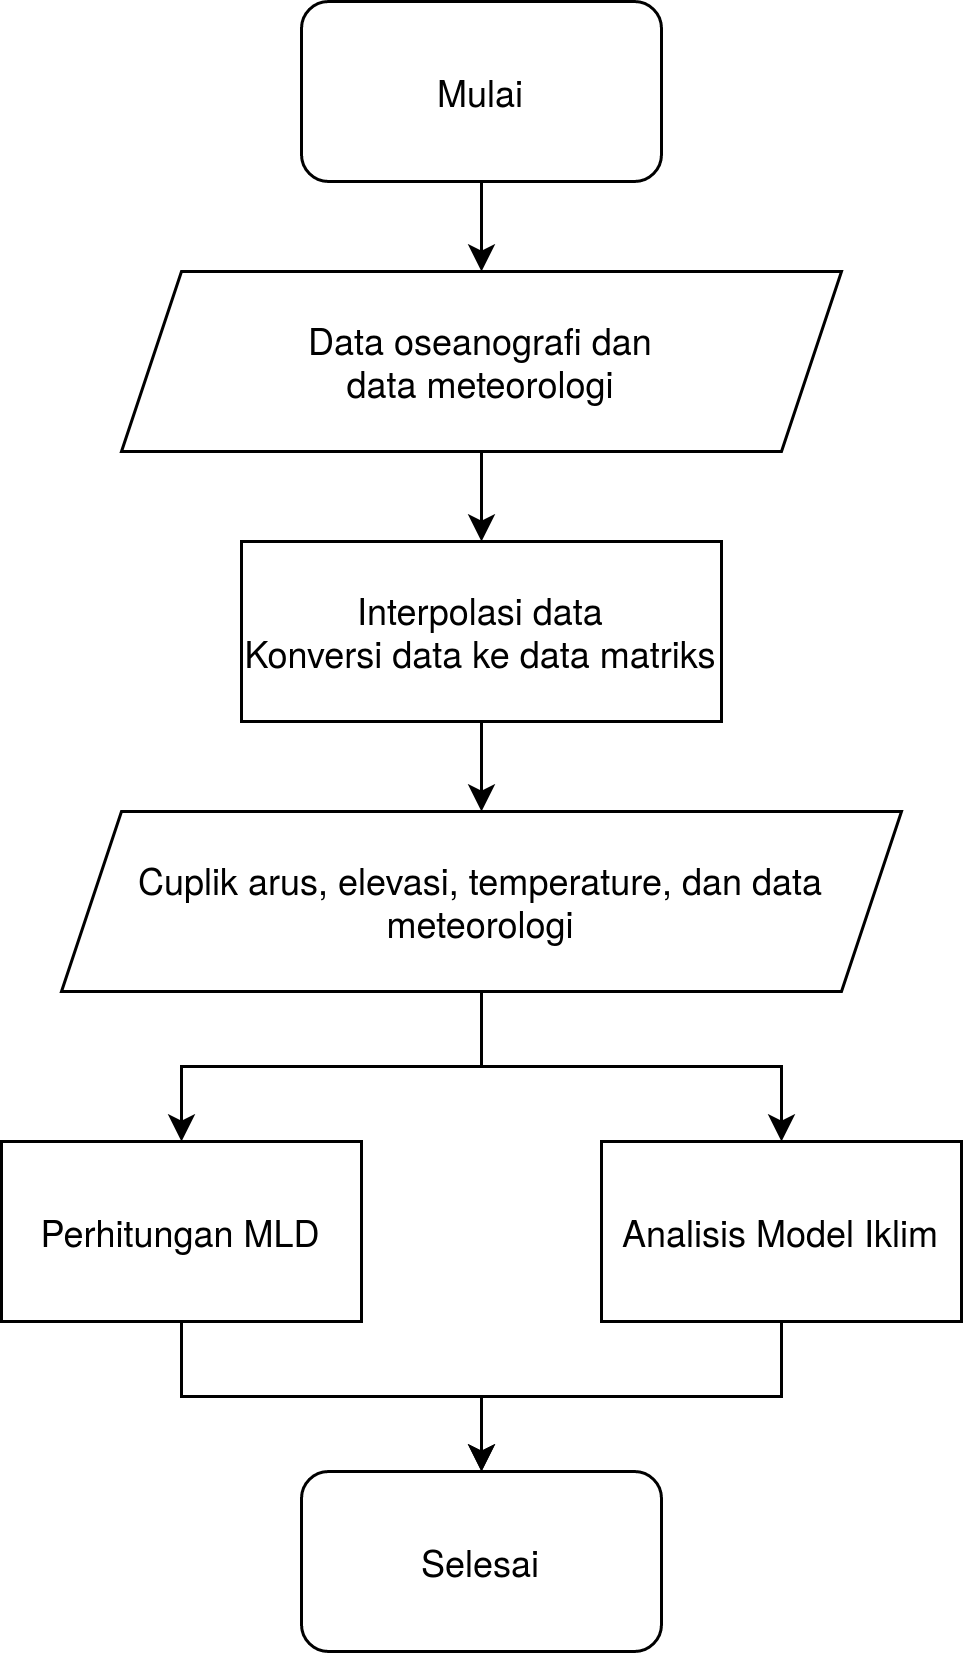
\includegraphics[width=7cm]{contents/flowchart.png}
		\caption{Diagram alir penelitian}
		\label{fig:flowchart}
	\end{figure}
	Prosedur penelitian mengikuti diagram alir pada Gambar \ref{fig:flowchart}. Data-data terkait penelitian didownload terlebih dahulu kemudian diinterpolasi untuk memenuhi data yang kosong serta untuk memperoleh resolusi spasial yang lebih detail. Selanjutnya data hasil interpolasi kemudian dibaca dan di konversi ke dalam data matriks pada MATLAB. Hasilnya adalah peta arus, elevasi, temperature, dan data meteorologi. Peta temperature kemudian diobservasi untuk menentukan kedalaman lapisan campuran selama 12 bulan. Sebagai verifikasi atas observasi kedalaman lapisan campuran, akan dilakukan analisis model iklim terhadap data meteorologi (\textit{2m air temperature, 2m specific humidity, convective precipitation rate, sea level pressure, wind stress U}, dan \textit{wind stress V}) selama 22 tahun dari tahun 2000 sampai 2021.
\end{spacing}
\vspace{-0.5pc}
\section[Jadwal Penelitian]{Jadwal Penelitian}
\begin{spacing}{1.5}
	Jadwal penelitian ditargetkan paling lama 7 bulan dengan rincian kegiatan disusun berdasarkan tabel berikut:
% Please add the following required packages to your document preamble:
% \usepackage{multirow}
	\begin{table}[htp]
		\centering
		\caption{Rencana jadwal pelaksanaan penelitian}
		\label{table:jadwal}
		\begin{tabular}{|c|c|ccccccc|}
			\hline
			\multirow{2}{*}{No.} & \multirow{2}{*}{Kegiatan} & \multicolumn{7}{c|}{Bulan}                                                                                                                            \\ \cline{3-9} 
			&                   & \multicolumn{1}{c|}{8} & \multicolumn{1}{c|}{9} & \multicolumn{1}{c|}{10} & \multicolumn{1}{c|}{11} & \multicolumn{1}{c|}{12} & \multicolumn{1}{c|}{1} &  2 \\ \hline 1
			& Studi literatur   & \multicolumn{1}{c|}{X} & \multicolumn{1}{c|}{X} & \multicolumn{1}{c|}{} & \multicolumn{1}{c|}{} & \multicolumn{1}{c|}{} & \multicolumn{1}{c|}{} &  \\ \hline 2
			& Seminar proposal    & \multicolumn{1}{c|}{X} & \multicolumn{1}{c|}{} & \multicolumn{1}{c|}{} & \multicolumn{1}{c|}{} & \multicolumn{1}{c|}{} & \multicolumn{1}{c|}{} &  \\ \hline 3
			& Pengumpulan data    & \multicolumn{1}{c|}{} & \multicolumn{1}{c|}{X} & \multicolumn{1}{c|}{} & \multicolumn{1}{c|}{} & \multicolumn{1}{c|}{} & \multicolumn{1}{c|}{} &  \\ \hline 4
			& Hasil dan analisis  & \multicolumn{1}{c|}{} & \multicolumn{1}{c|}{} & \multicolumn{1}{c|}{X} & \multicolumn{1}{c|}{X} & \multicolumn{1}{c|}{} & \multicolumn{1}{c|}{} &  \\ \hline 5
			& Seminar hasil       & \multicolumn{1}{c|}{} & \multicolumn{1}{c|}{} & \multicolumn{1}{c|}{} & \multicolumn{1}{c|}{} & \multicolumn{1}{c|}{X} & \multicolumn{1}{c|}{} &  \\ \hline 6
			& Ujian sidang        & \multicolumn{1}{c|}{} & \multicolumn{1}{c|}{} & \multicolumn{1}{c|}{} & \multicolumn{1}{c|}{} & \multicolumn{1}{c|}{} & \multicolumn{1}{c|}{X} &  \\ \hline 7
			& Publikasi           & \multicolumn{1}{c|}{} & \multicolumn{1}{c|}{} & \multicolumn{1}{c|}{} & \multicolumn{1}{c|}{} & \multicolumn{1}{c|}{} & \multicolumn{1}{c|}{X} & X  \\ \hline 
		\end{tabular}
	\end{table}

\end{spacing}